\appendix

\section{Decadal integration: detailed verification}
\label{app:multiyear}

This appendix collects the detailed verification of the ten-year
autonomous CMFD integration (2009--2018) summarized in
Sect.~\ref{sec:multiyear}. Both implementations use the same shared initial
state; each year is restarted from the terminal state of the previous year,
and the final forcing records of each annual file are linked to the first
records of the following year, so that the interpolated forcing is
continuous at each year boundary. The Fortran reference integrates each year
in the offline configuration, restarted from the previous year's terminal
state; the PyTorch implementation carries the state in memory across the
same year boundaries. States are archived every ten days and at each annual
terminal step.

The offline forcing alignment must be replicated exactly rather than
approximately. When a variant of the PyTorch implementation samples the state meteorology
at the raw three-hourly records instead of at the linearly interpolated
physics-step boundaries (radiation and precipitation held at the next
record, as in the reference configuration), the domain-RMSE soil-temperature
difference reaches $2.1\times10^{-1}$~K within ten days and isolated snow
columns accumulate over $10^{2}$~kg~m$^{-2}$ of spurious snow water
equivalent within the first year, even though the underlying forcing data
are identical. All successively restarted results use the exact reference alignment.

\begin{table}[H]
\caption{Terminal day-3652 (31 December 2018) Fortran--PyTorch comparison for
the ten-year autonomous CMFD integration. Relative RMSE is normalized
by the root-mean-square Fortran field over the stated mask. ``All'' contains
97,709 columns; the resolved-snow mask (snow-cover fraction above
$10^{-3}$) contains 82,132 columns at day~3652.}
\label{tab:multiyear-autonomous}
\centering
\small
\begin{tabular}{llrr}
\hline
Quantity (unit) & mask & RMSE & relative RMSE (\%) \\
\hline
Soil temperature, layer 1 (K) & all & $8.05\times10^{-4}$ & $3.06\times10^{-4}$ \\
Soil temperature, layer 2 (K) & all & $7.09\times10^{-4}$ & $2.67\times10^{-4}$ \\
Soil temperature, layer 3 (K) & all & $6.12\times10^{-4}$ & $2.25\times10^{-4}$ \\
Soil temperature, layer 4 (K) & all & $6.81\times10^{-4}$ & $2.44\times10^{-4}$ \\
Soil water, layer 1 (kg m$^{-2}$) & all & $4.24\times10^{-3}$ & $2.46\times10^{-2}$ \\
Soil water, layer 2 (kg m$^{-2}$) & all & $8.86\times10^{-3}$ & $1.66\times10^{-2}$ \\
Soil water, layer 3 (kg m$^{-2}$) & all & $2.45\times10^{-2}$ & $1.28\times10^{-2}$ \\
Soil water, layer 4 (kg m$^{-2}$) & all & $6.36\times10^{-2}$ & $1.19\times10^{-2}$ \\
Snow water equivalent (kg m$^{-2}$) & resolved snow & $8.39\times10^{-3}$ & $2.38\times10^{-3}$ \\
Snow temperature (K) & resolved snow & $1.06\times10^{-3}$ & $4.21\times10^{-4}$ \\
Snow density (kg m$^{-3}$) & resolved snow & $1.59\times10^{-2}$ & $1.11\times10^{-2}$ \\
Snow albedo (--) & resolved snow & $1.26\times10^{-5}$ & $2.18\times10^{-3}$ \\
\hline
\end{tabular}
\end{table}

The error level of an individual annual terminal is set by the forcing
realization rather than by the experiment design. The successively restarted integration
starts from the same common spun-up initial state as the one-year experiment of
Sect.~\ref{sec:annual-autonomous-equivalence}, under the 2009 forcing
instead of the 2018 forcing: at its first-year terminal (day~365 of 2009)
the layer-1 soil-temperature RMSE is $6.1\times10^{-4}$~K, 2.2~times
\emph{larger} than the one-year value of
Table~\ref{tab:annual-autonomous}, while the layer-4 soil-water RMSE is
$3.3\times10^{-2}$~kg~m$^{-2}$ ($6.3\times10^{-3}$~\% relative), six times
\emph{larger} than the one-year value ($5.6\times10^{-3}$~kg~m$^{-2}$,
$1.0\times10^{-3}$~\%). With identical code and initial state, this spread
measures the realization dependence of the round-off-seeded branch
selection, which phase, density, or stability thresholds a given year's
weather crosses, and it is of the same size as the year-to-year
oscillation of Fig.~\ref{fig:multiyear-error-growth} itself. No single
annual terminal is therefore ``the'' translation error of the autonomous
configuration; the bounded envelope across the decade is.

Three observations support the branch-event reading summarized in
Sect.~\ref{sec:multiyear}. First, each field's error peaks in its own
threshold-active season: layer-1 soil-temperature RMSE peaks in July at
$1.5\times10^{-2}$~K, eight times its January minimum; snow-water RMSE peaks
in the March melt season nearly two orders of magnitude above its summer
minimum; the layer-4 soil water and temperature errors peak in
October--November, the lagged integral of the summer evaporation season.
Second, the annual-terminal errors rise until the 2012--2014 terminals and
then decline (a log$_{10}$ slope of $-0.2$ to $-0.5$ per decade), and each
year's terminal error correlates with that year's persistent snow-cover
extent ($r=+0.82$ for layer-4 soil temperature and $r=+0.75$ for layer-4
soil water against the annual snow-covered column--days), so the peak
years are those with the most persistent snow cover. Third, the columns
carrying the largest layer-1 soil-temperature error are mostly snow-free
(median snow water $0.0$~kg~m$^{-2}$; snow involved in 29~\% of records),
which locates the summer maxima in soil-moisture branch activity rather
than in snow.

\begin{figure}[H]
\centering

\includegraphics[width=\linewidth]{figures/multiyear_gpunative/multiyear_annual_terminal_error_growth.png}
\caption{Fortran--PyTorch errors at the ten annual (31~December) terminal
states of the successively restarted 2009--2018 integration, on logarithmic axes. Top row:
soil temperature (layers 1--4) and soil water (layers 1--4) over all
columns. Bottom row: snow water equivalent over all columns, and snow
temperature, density, and albedo over the resolved-snow mask (snow-cover
fraction above $10^{-3}$). Left column: RMSE in native units; right column:
relative RMSE.}
\label{fig:multiyear-error-growth}
\end{figure}

\begin{figure}[H]
\centering
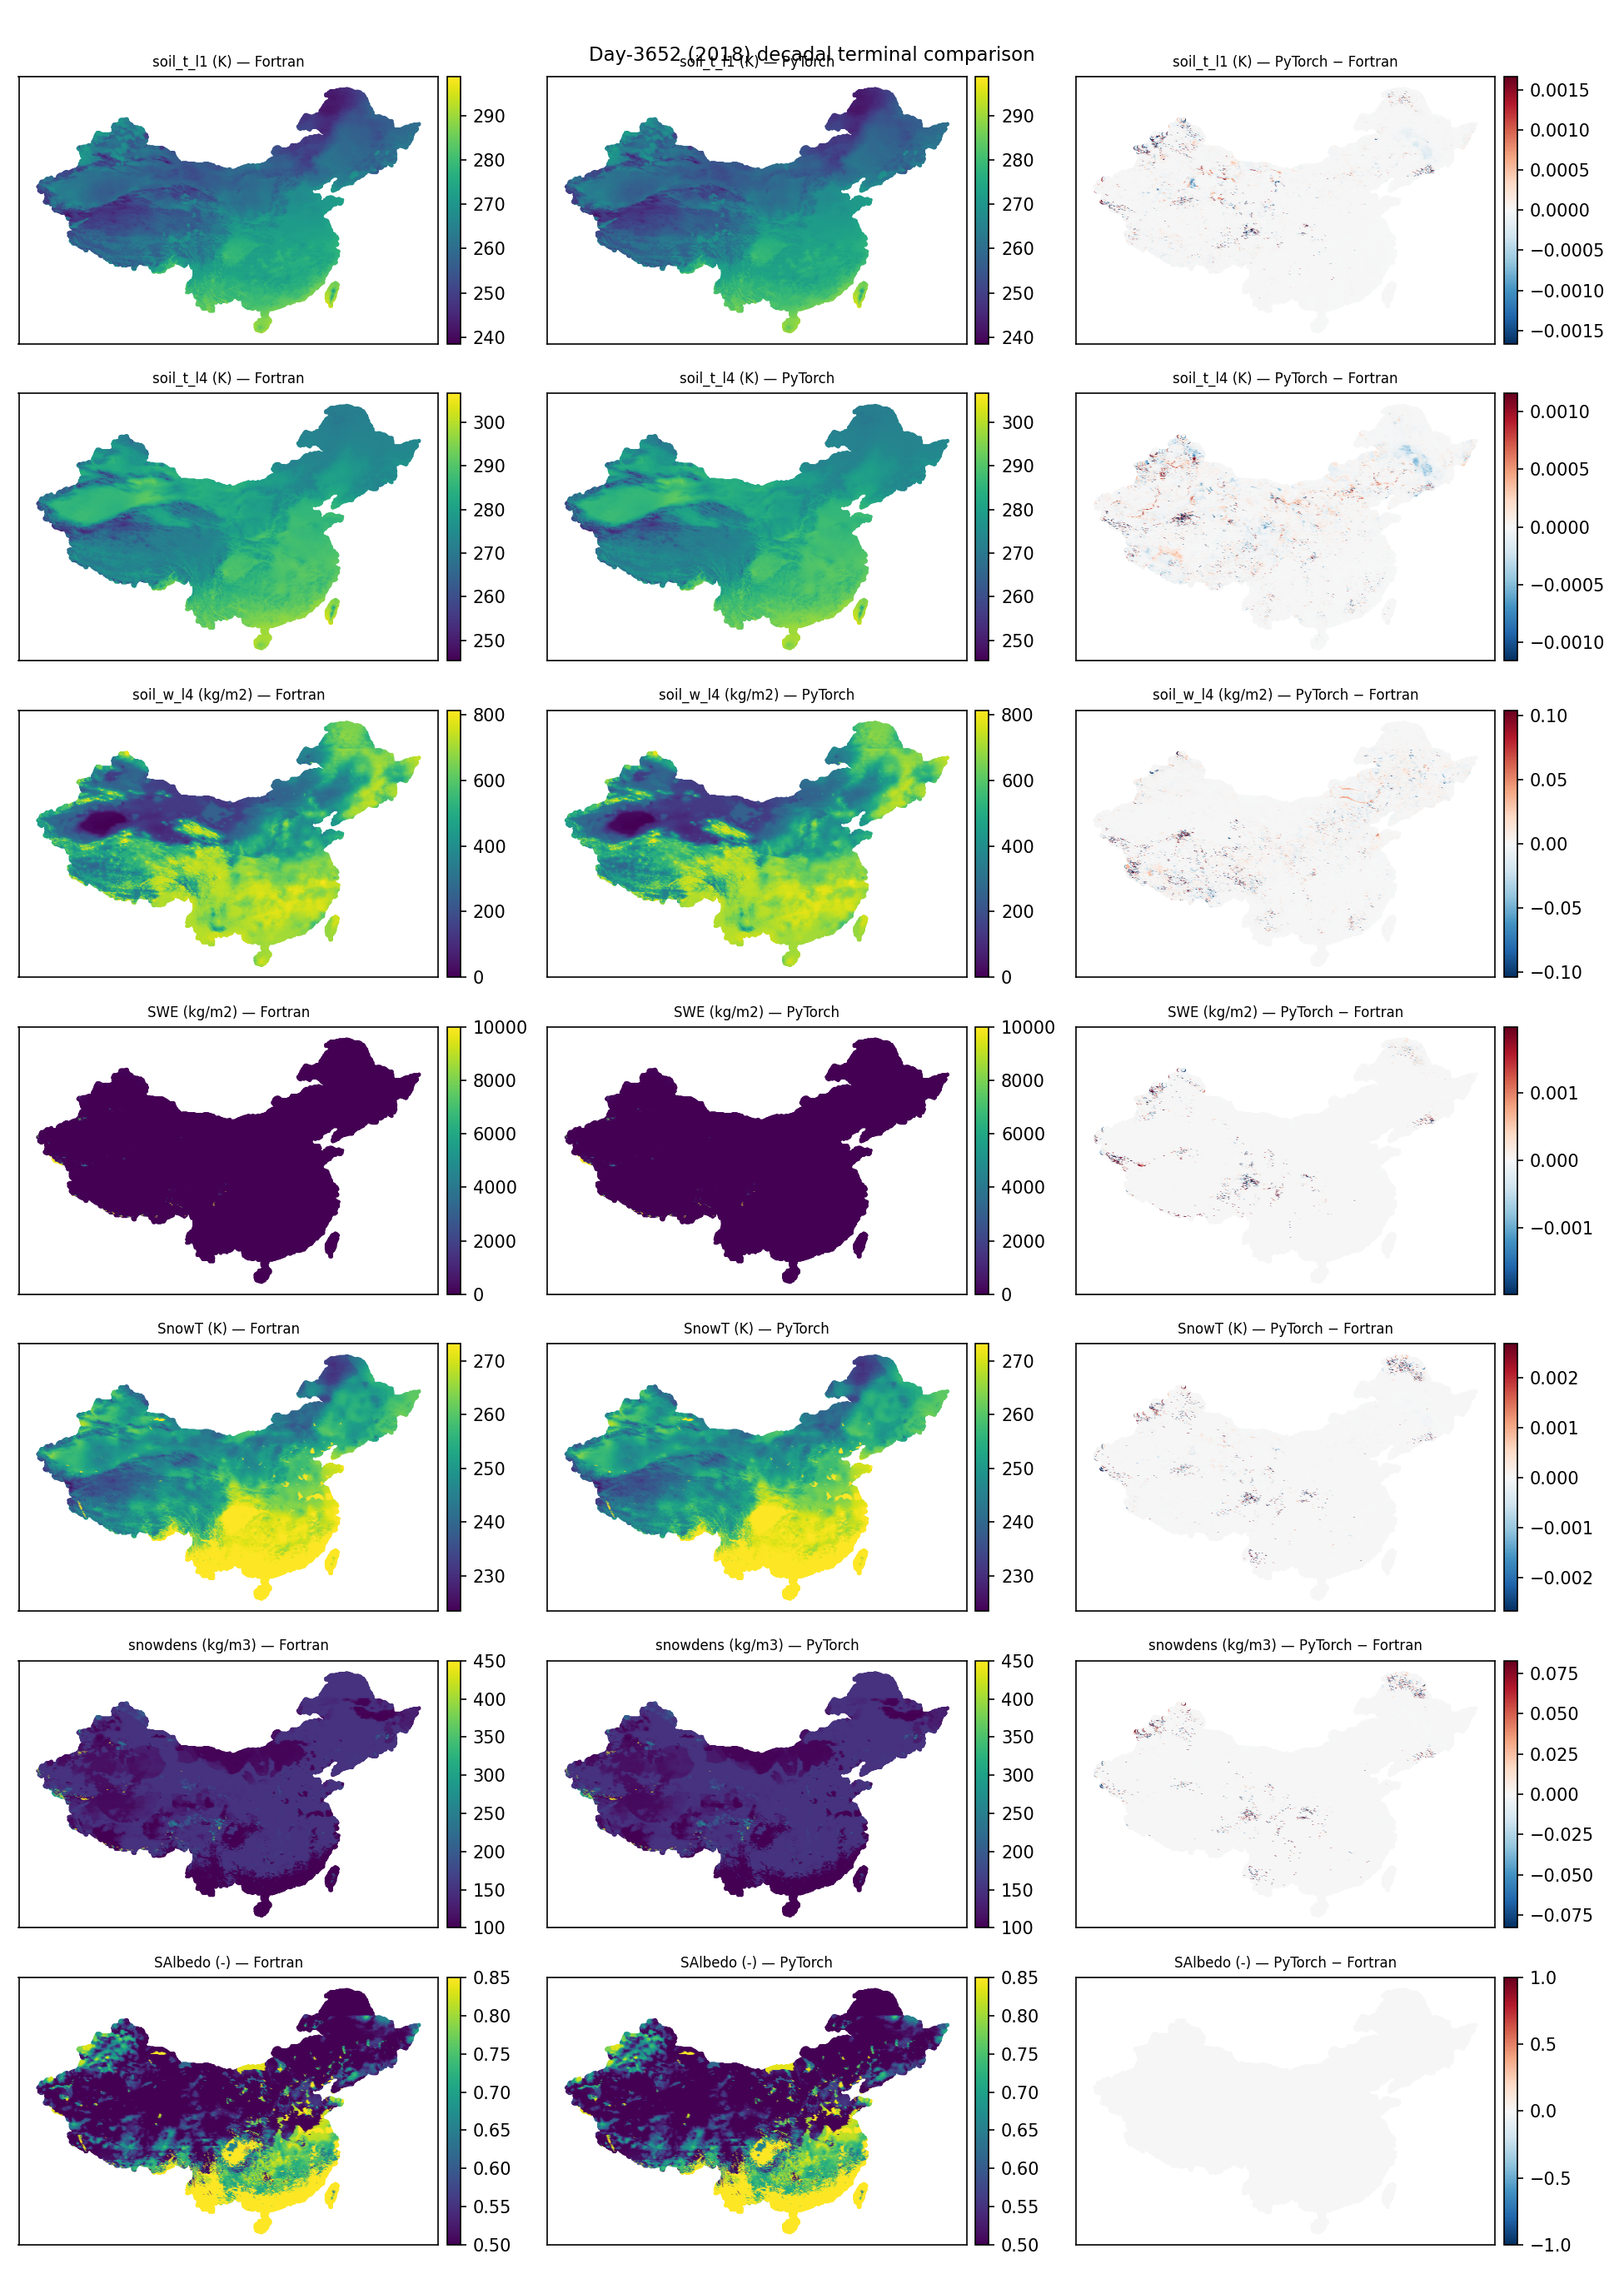
\includegraphics[width=\linewidth]{figures/multiyear_gpunative/multiyear_terminal_maps.png}
\caption{Day-3652 (31~December 2018) decadal terminal comparison on the CMFD
grid. Each row is one field (soil temperature layers 1 and 4, soil water
layer 4, snow water equivalent, snow temperature, density, and albedo);
columns show the Fortran state, the PyTorch state, and the signed
PyTorch-minus-Fortran difference. Difference colour limits use the 99.5th
percentile of the absolute error.}
\label{fig:multiyear-terminal-maps}
\end{figure}

